\documentclass[a4paper]{article}
\usepackage[margin=1.0in]{geometry}
\usepackage{amsmath,amssymb,bm,bbm}
\usepackage{enumitem,array}
\usepackage{multirow,graphicx,float}
\usepackage{type1ec,type1cm,psfrag,dvipscol,dvipaste,dvips}
\newcommand\showrowno{\stepcounter{rowno}\therowno}

\title{cs224n Assignment \#3}
\date{}
\author{}

\begin{document}

\begin{center}
    \section*{cs224n Assignment \#4}
\end{center}
\medskip

% \maketitle

\subsection*{1. Neural Machine Translation with RNNs}

    \begin{enumerate}[label=(\alph*)]
        \setcounter{enumi}{6}        
        \item abc

        \setcounter{enumi}{8}
        \item Training and Test Results
        \begin{figure}[h]
            \centering
            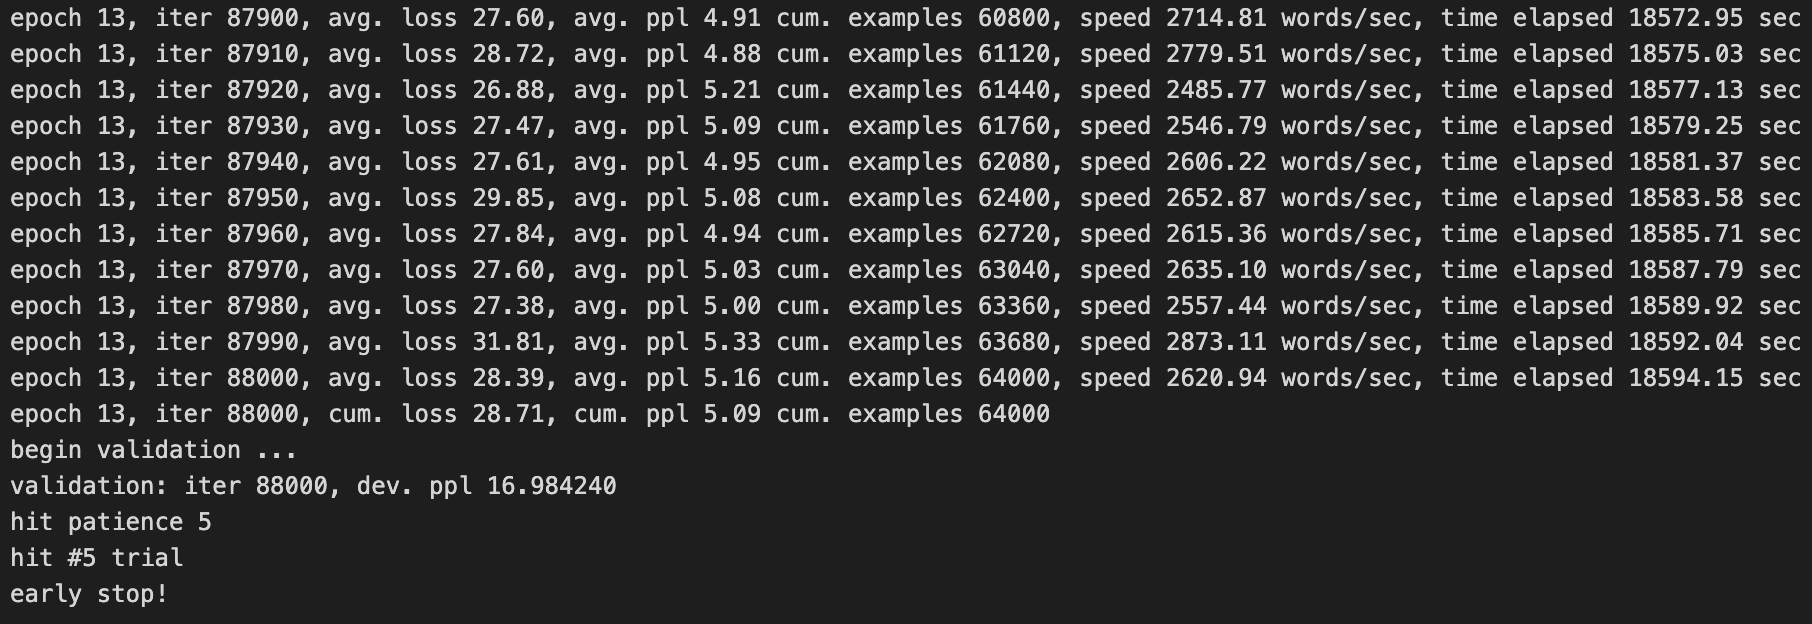
\includegraphics[width=0.7\textwidth]{NMT_train_complete.png}
            % \caption{test UAS after 10 epochs}
            \label{fig:training completed after 5 hours}
        \end{figure}
        
        \begin{figure}[h]
            \centering
            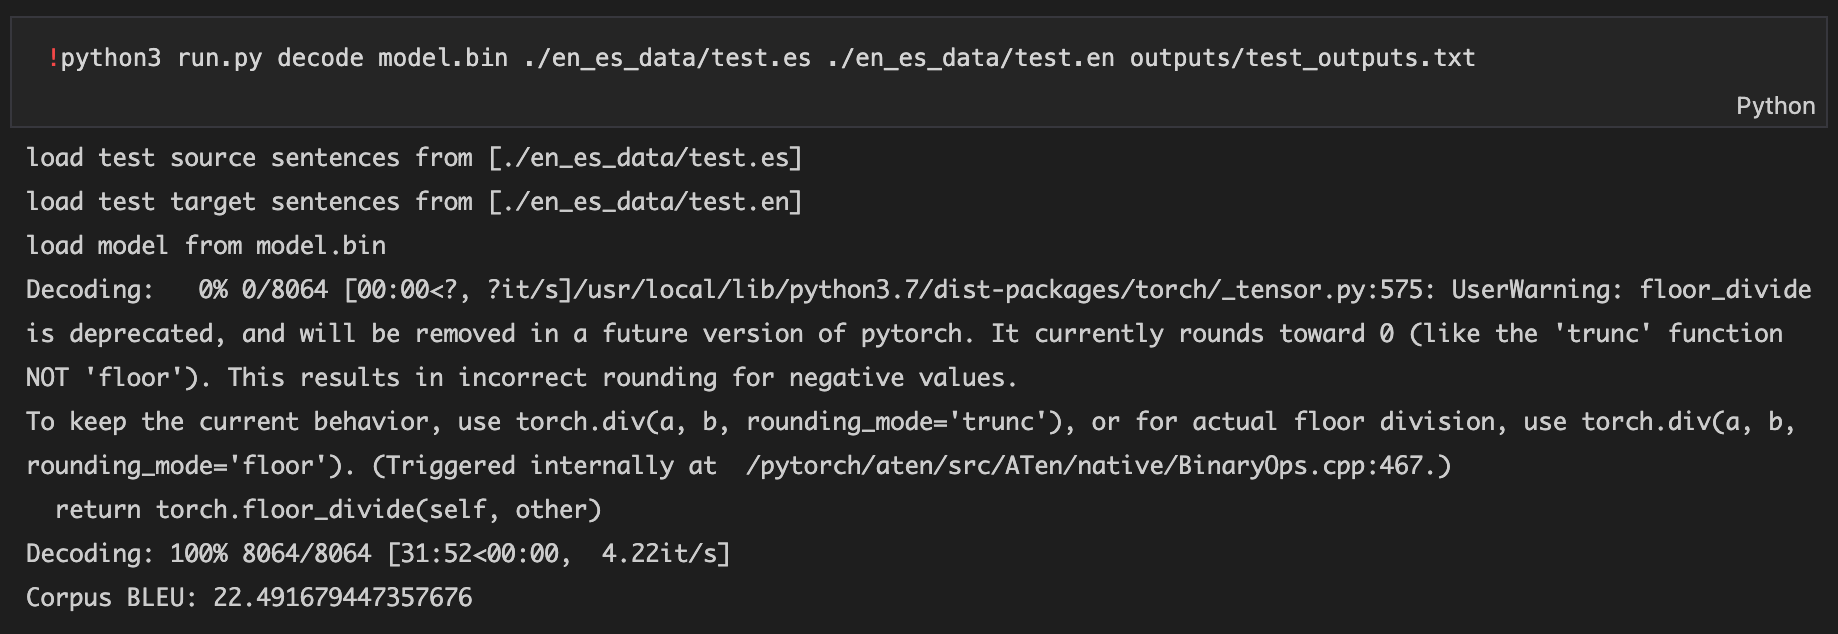
\includegraphics[width=0.7\textwidth]{NMT_BLEU_22.49.png}
            % \caption{Not bad, above 21}
            \label{fig:BLEU score 22.49}
        \end{figure}

        final BLEU score: 22.49
        
        \item 
        \begin{enumerate}[label=\roman*.]
            \item dot product attention ($\mathbf{e}_{t,i}=\mathbf{s}_{t}^{\mathsf{T}}\mathbf{h}_{i}$)
            \begin{itemize}
                \item advantage: It's easy and efficient to compute the attention.
                \item disadvantage: It has less flexibility and it can be used only when dimensions are the same for both vectors.
            \end{itemize}

            \item multiplicative attention ($\mathbf{e}_{t,i}=\mathbf{s}_{t}^{\mathsf{T}}\mathbf{W}\mathbf{h}_{i}$)
            \begin{itemize}
                \item advantage: It can get some flexibility through weight matrix and it can be calculated even though the column lengths are different between two vectors.
                \item disadvantage: It needs two expensive matrix multiplications to get one attention element.
            \end{itemize}

            \item additive attention ($\mathbf{e}_{t,i}=\mathbf{v}^{\mathsf{T}}(\mathbf{W}_{1}\mathbf{h}_{i}+\mathbf{W}_{2}\mathbf{s}_{t})$)
            \begin{itemize}
                \item advantage: As using different weights for two vectors, it is possible to have more flexibility on calculating attention.
                \item disadvantage: It is much slower than two above methods with two matrix multiplications and it ignores the relation between $\mathbf{h}$ and $\mathbf{s}$.
            \end{itemize}

        \end{enumerate}
    \end{enumerate}

\subsection*{2. Analyzing NMT Systems}

    \begin{enumerate}[label=(\alph*)]
        \setcounter{enumi}{0} 
        \item Analyzing errors in the outputs of NMT model
        
        \begin{enumerate}[label=\roman*.]
            \item
            Source Sentence: \textit{Aquí otro de mis favoritos, “La noche estrellada”.} 

            Reference Translation: \textit{So another one of my favorites, “The Starry Night”.}

            NMT Translation: \textit{Here’s another favorite of my favorites, “The Starry Night”.}

            \begin{enumerate}[label=\arabic*.]
                \item Identify the error: Here’s another favorite of my favorites $\rightarrow$ So another one of my favorites
                \item Provide a reason: 
                \item Describe a possible way to fix the error: 
            \end{enumerate}
            
            \item
            Source Sentence: \textit{Ustedes saben que lo que yo hago es escribir para los niños, y, de hecho, probablemente soy el autor para niños, mas ledo en los EEUU.}

            Reference Translation: \textit{You know, what I do is write for children, and I’m probably America’s most widely read children’s author, in fact.}
            
            NMT Translation: \textit{You know what I do is write for children, and in fact, I’m probably the author for children, more reading in the U.S.}
            
            \begin{enumerate}[label=\arabic*.]
                \item Identify the error: America’s most widely read children’s author, in fact. $\rightarrow$ the author for children, more reading in the U.S.
                \item Provide a reason: spanish word 'mas' has two meanings, more and most. Choosing between two makes the translation difference.
                \item Describe a possible way to fix the error: 
            \end{enumerate}
            
            \item
            Source Sentence: \textit{Un amigo me hizo eso – Richard \underline{Bolingbroke}.}
            
            Reference Translation: \textit{A friend of mine did that – Richard \underline{Bolingbroke}.}
            
            NMT Translation: \textit{A friend of mine did that – Richard <unk>}
            
            \begin{enumerate}[label=\arabic*.]
                \item Identify the error: <unk> $\rightarrow$ \underline{Bolingbroke} 
                \item Provide a reason: 
                \item Describe a possible way to fix the error: just copy the word if the word is unlisted in dictionary.
            \end{enumerate}
            
            \item
            
            Source Sentence: \textit{Solo tienes que dar vuelta a la manzana para verlo como una epifanía.}
            
            Reference Translation: \textit{You’ve just got to go around the block to see it as an epiphany.} 
            
            NMT Translation: \textit{You just have to go back to the apple to see it as a epiphany.}
            
            \begin{enumerate}[label=\arabic*.]
                \item Identify the error: go back to the apple $\rightarrow$ go around the block
                \item Provide a reason: spanish word 'manzana' has two meanings, apple and block.
                \item Describe a possible way to fix the error: the model should be able to distinguish where the word is used in different contexts 
            \end{enumerate} 
            
            \item
            
            Source Sentence: \textit{Ella salvó mi vida al permitirme entrar al baño de la sala de profesores.}
            
            Reference Translation: \textit{She saved my life by letting me go to the bathroom in the teachers’ lounge.}
            
            NMT Translation: \textit{She saved my life by letting me go to the bathroom in the women’s room.}
            
            \begin{enumerate}[label=\arabic*.]
                \item Identify the error: in the women’s room $\rightarrow$ in the teachers’ lounge
                \item Provide a reason: 
                \item Describe a possible way to fix the error: 
            \end{enumerate}
            
            \item
            
            Source Sentence: \textit{Eso es más de 100,000 hectáreas.} 
            
            Reference Translation: \textit{That’s more than 250 thousand acres.}
            
            NMT Translation: \textit{That’s over 100,000 acres.}
            
            \begin{enumerate}[label=\arabic*.]
                \item Identify the error: 100,000 acres $\rightarrow$ 250 thousand acres
                \item Provide a reason: The model lacks of ability to convert units (1 hectare \eqsim 2.47 acres)
                \item Describe a possible way to fix the error: 
            \end{enumerate}

        \end{enumerate}   

        \item Errors that my model produced 

        \begin{enumerate}[label=\roman*.]

            \item example 1
            
            \begin{enumerate}[label=\arabic*.]
            
                \item Source Sentence: \textit{Necesita verdad y belleza, y estoy muy felz que hoy se habl mucho de esto.} 
                \item Reference Translation: \textit{It needs truth and beauty,  and I'm so happy it's been mentioned so much here today.}
                \item NMT Translation: \textit{It needs truth and beauty, and I'm very happy that I talked a lot about this.}
                \item Identify the error: I talked a lot about this. $\rightarrow$ it's been mentioned so much here today.
                \item Provide a reason: The model absorbed the mea
                \item Describe a possible way to fix the error: 
            \end{enumerate}

            \item example 2
            
            Source Sentence: \textit{Otros equipos decidieron imitarlos.} 
            
            Reference Translation: \textit{Other teams followed suit.}
            
            NMT Translation: \textit{Other teams decided to be <unk>}
            
            \begin{enumerate}[label=\arabic*.]
                \item Identify the error: decided to be <unk> $\rightarrow$ followed suit
                \item Provide a reason: The model lacks an ability to understand how the compound word is made of (imitarlos = imitar + los)
                \item Describe a possible way to fix the error: let the model understand the fertile words (the words that produce several corresponding word--one-to-many)
            \end{enumerate}

        \end{enumerate}  

        \item BLEU score
    
        \begin{enumerate}[label=\roman*.]

            \item Calculate actual BLEU score(Bilingual Evaluation Understudy Score)
            
            \begin{itemize} 
                \item n-gram score on $\mathbf{c}_{1}$ 
                \begin{table}[h]
                    % \newcounter{rowno}
                    % \setcounter{rowno}{0}
                    \begin{tabular}{c|c|c|c|c|c}
                        % \noalign{\smallskip}\noalign{\smallskip}
                        ngram & token & $\text{Count}_{\mathbf{r}_{1}}(\text{ngram})$ & $\text{Count}_{\mathbf{r}_{2}}(\text{ngram})$ 
                        & $\text{Count}_{\mathbf{c}_{1}}(\text{ngram})$ & $\min(\underset{i=1, 2}{\max}\text{Count}_{\mathbf{r}_{i}}, \text{Count}_{\mathbf{c}_{1}}) (= A)$ \\
                        \hline
                        \multirow{5}{*}{unigram} & the & 0 & 0 & 1 & 0 \\
                        & love & 1 & 1 & 1 & 1 \\
                        & can & 1 & 0 & 1 & 1 \\
                        & always & 1 & 0 & 1 & 1 \\ 
                        & do & 0 & 0 & 1 & 0 \\ 
                        \hline \hline
                        \multirow{4}{*}{bigram} & the love & 0 & 0 & 1 & 0 \\ 
                        & love can & 1 & 0 & 1 & 1 \\ 
                        & can always & 1 & 0 & 1 & 1 \\ 
                        & always do & 0 & 0 & 1 & 0 \\ 
                    \end{tabular}
                \end{table} 
                \begin{flalign*}
                    p_1&= \dfrac{\sum_{\text{unigram} \in \textbf{c}}A}{\sum_{\text{unigram} \in \textbf{c}}\text{Count}_{\mathbf{c}_{1}}}=\dfrac{3}{5}\\ 
                    p_2&= \dfrac{\sum_{\text{bigram} \in \textbf{c}}A}{\sum_{\text{bigram} \in \textbf{c}}\text{Count}_{\mathbf{c}_{1}}}=\dfrac{2}{4}&
                \end{flalign*}
                $c$ (the length of $\mathbf{c}_{1}$) = 5, $r^{*}$ (the length of $\mathbf{r}$ closest to $c$) = 5. $\therefore BP = 1$
                \begin{flalign*}
                    \therefore BLEU&= BP \times \exp(\sum_{n=1}^{4} \lambda_{n}\log p_{n}) \\ 
                    &= 1 \times \exp(0.5 \cdot \log(\dfrac{3}{5}) + 0.5 \cdot \log(\dfrac{2}{4}) ) =  0.7699 &
                \end{flalign*}

                \item n-gram score on $\mathbf{c}_{2}$ 
                \begin{table}[h]
                    % \newcounter{rowno}
                    % \setcounter{rowno}{0}
                    \begin{tabular}{c|c|c|c|c|c}
                        % \noalign{\smallskip}\noalign{\smallskip}
                        ngram & token & $\text{Count}_{\mathbf{r}_{1}}(\text{ngram})$ & $\text{Count}_{\mathbf{r}_{2}}(\text{ngram})$ 
                        & $\text{Count}_{\mathbf{c}_{2}}(\text{ngram})$ & $\min(\underset{i=1, 2}{\max}\text{Count}_{\mathbf{r}_{i}}, \text{Count}_{\mathbf{c}_{2}})$ \\
                        \hline
                        \multirow{5}{*}{unigram} & love & 1 & 1 & 1 & 1 \\
                        & can & 1 & 0 & 1 & 1 \\
                        & make & 0 & 0 & 1 & 0 \\                         
                        & anything & 0 & 1 & 1 & 1 \\ 
                        & possible & 0 & 1 & 1 & 1 \\ 
                        \hline \hline
                        \multirow{4}{*}{bigram} & love can & 1 & 0 & 1 & 1 \\ 
                        & can make & 0 & 0 & 1 & 0 \\ 
                        & make anything & 0 & 0 & 1 & 0 \\ 
                        & anything possible & 0 & 1 & 1 & 1 \\ 
                    \end{tabular}
                \end{table}
                \begin{flalign*}
                    p_1&= \dfrac{\sum_{\text{unigram} \in \textbf{c}}A}{\sum_{\text{unigram} \in \textbf{c}}\text{Count}_{\mathbf{c}_{2}}}=\dfrac{4}{5}\\ 
                    p_2&= \dfrac{\sum_{\text{bigram} \in \textbf{c}}A}{\sum_{\text{bigram} \in \textbf{c}}\text{Count}_{\mathbf{c}_{2}}}=\dfrac{2}{4}&
                \end{flalign*}
                $c$ (the length of $\mathbf{c}_{2}$) = 5, $r^{*}$ (the length of $\mathbf{r}$ closest to $c$) = 5. $\therefore BP = 1$
                \begin{flalign*}
                    \therefore BLEU &= BP \times \exp(\sum_{n=1}^{4} \lambda_{n}\log p_{n}) \\ 
                    &= 1 \times \exp(0.5 \cdot \log(\dfrac{4}{5}) + 0.5 \cdot \log(\dfrac{2}{4}) ) =  0.8196 &
                \end{flalign*} 
                Comparing BLEU scores on two candidates, $\mathbf{c}_{2}$ is considered the better translation and I can intuitively agree with it.
                                
            \end{itemize} 

            \item In the situation that there exists only one Reference Translation $\mathbf{r}_{1}$
            
            \begin{itemize} 
                \item n-gram score on $\mathbf{c}_{1}$ 
                \begin{table}[h]
                    % \newcounter{rowno}
                    % \setcounter{rowno}{0}
                    \begin{tabular}{c|c|c|c|c}
                        % \noalign{\smallskip}\noalign{\smallskip}
                        ngram & token & $\text{Count}_{\mathbf{r}_{1}}(\text{ngram})$ 
                        & $\text{Count}_{\mathbf{c}_{1}}(\text{ngram})$ & $\min(\text{Count}_{\mathbf{r}_{1}}, \text{Count}_{\mathbf{c}_{1}}) (= A)$ \\
                        \hline
                        \multirow{5}{*}{unigram} & the & 0 & 1 & 0 \\
                        & love & 1 & 1 & 1 \\
                        & can & 1 & 1 & 1 \\
                        & always & 1 & 1 & 1 \\ 
                        & do & 0 & 1 & 0 \\ 
                        \hline \hline
                        \multirow{4}{*}{bigram} & the love & 0 & 1 & 0 \\ 
                        & love can & 1 & 1 & 1 \\ 
                        & can always & 1 & 1 & 1 \\ 
                        & always do & 0 & 1 & 0 \\ 
                    \end{tabular}
                \end{table} 
                \begin{flalign*}
                    p_1&= \dfrac{\sum_{\text{unigram} \in \textbf{c}}A}{\sum_{\text{unigram} \in \textbf{c}}\text{Count}_{\mathbf{c}_{1}}}=\dfrac{3}{5}\\ 
                    p_2&= \dfrac{\sum_{\text{bigram} \in \textbf{c}}A}{\sum_{\text{bigram} \in \textbf{c}}\text{Count}_{\mathbf{c}_{1}}}=\dfrac{2}{4}&
                \end{flalign*}
                $c$ (the length of $\mathbf{c}_{1}$) = 5, $r^{*}$ (the length of $\mathbf{r}$ closest to $c$) = 5. $\therefore BP = 1$
                \begin{flalign*}
                    \therefore BLEU&= BP \times \exp(\sum_{n=1}^{4} \lambda_{n}\log p_{n}) \\ 
                    &= 1 \times \exp(0.5 \cdot \log(\dfrac{3}{5}) + 0.5 \cdot \log(\dfrac{2}{4}) ) =  0.7699 &
                \end{flalign*}

                \item n-gram score on $\mathbf{c}_{2}$ 
                \begin{table}[h]
                    % \newcounter{rowno}
                    % \setcounter{rowno}{0}
                    \begin{tabular}{c|c|c|c|c}
                        % \noalign{\smallskip}\noalign{\smallskip}
                        ngram & token & $\text{Count}_{\mathbf{r}_{1}}(\text{ngram})$ 
                        & $\text{Count}_{\mathbf{c}_{2}}(\text{ngram})$ & $\min(\text{Count}_{\mathbf{r}_{1}}, \text{Count}_{\mathbf{c}_{2}}) (= A)$ \\
                        \hline
                        \multirow{5}{*}{unigram} & love & 1 & 1 & 1 \\
                        & can & 1 & 1 & 1 \\
                        & make & 0 & 1 & 0 \\                         
                        & anything & 0 & 1 & 0 \\ 
                        & possible & 0 & 1 & 0 \\ 
                        \hline \hline
                        \multirow{4}{*}{bigram} & love can & 1 & 1 & 1 \\ 
                        & can make & 0 & 1 & 0 \\ 
                        & make anything & 0 & 1 & 0 \\ 
                        & anything possible & 0 & 1 & 0 \\ 
                    \end{tabular}
                \end{table}
                \begin{flalign*}
                    p_1&= \dfrac{\sum_{\text{unigram} \in \textbf{c}}A}{\sum_{\text{unigram} \in \textbf{c}}\text{Count}_{\mathbf{c}_{2}}}=\dfrac{2}{5}\\ 
                    p_2&= \dfrac{\sum_{\text{bigram} \in \textbf{c}}A}{\sum_{\text{bigram} \in \textbf{c}}\text{Count}_{\mathbf{c}_{2}}}=\dfrac{1}{4}&
                \end{flalign*}
                $c$ (the length of $\mathbf{c}_{2}$) = 5, $r^{*}$ (the length of $\mathbf{r}$ closest to $c$) = 5. $\therefore BP = 1$
                \begin{flalign*}
                    \therefore BLEU &= BP \times \exp(\sum_{n=1}^{4} \lambda_{n}\log p_{n}) \\ 
                    &= 1 \times \exp(0.5 \cdot \log(\dfrac{2}{5}) + 0.5 \cdot \log(\dfrac{1}{4}) ) =  0.6065 &
                \end{flalign*}
                Comparing BLEU scores on two candidates, the result gets reversed and $\mathbf{c}_{1}$ is considered the better translation, which is counterintuitive.
                                
            \end{itemize}

            \item Language translation is a subjective field and there is no right answer on translating certain sentence.
            Therefore, bilingual translator could miss the subtle sense from the sentence or the better words for the corresponding sentence. 
            In that sense, even better translation could get lower BLEU score with single reference translation like above.
            Measuring NMT performance based on BLEU scale needs a large set of reference translation.

            \item 
            
            \begin{itemize} 
                \item Adventages: 
                
                1) BLEU score is objective comparing to human measure so that it's simple and efficient to compute by computing resources. 
                
                2) From its efficiency on computing with proper reference translation, BLEU score can be used as efficient loss function to optimize neural network.
                \item Disadvantages: 
                
                1) phrase order or position aren't counted when calculating BLEU score. 
                
                2) if single translation is used as the only reference, the credibility of BLEU score gets lower due to the reason described above.
            \end{itemize}

        \end{enumerate}    

    \end{enumerate}

\end{document} 